\newpage
\hypertarget{treeToModel vis}{}
\subsection{Vis Tree to Model Source}
\visHeader

First transformation: take the parent \texttt{myLibrary} folder and create a library from it.
Second transformation: take the \emph{english} and \texttt{french} subfolders, and turn them into different shelves in the library.

\begin{itemize}

\item[$\blacktriangleright$] Select the \texttt{Rules} folder in the project browser, and click to create a new rule. Name it \texttt{FolderToLibrary}, and
complete it as depicted in Fig.~\ref{ea:FolderIntoLibrary_Complete} with the correspondence type established when we first created the TGG schema.

\vspace{0.5cm}

\begin{figure}[htbp]
\begin{center}
  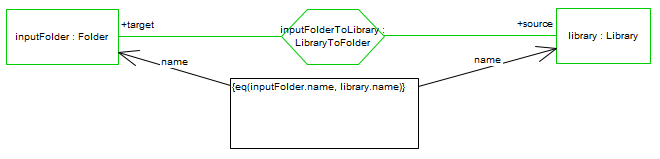
\includegraphics[width=\textwidth]{ea_completeFolderIntoLibrary}
  \caption{completed folder into library}
  \label{ea:FolderIntoLibrary_Complete}
\end{center}
\end{figure}

\item[$\blacktriangleright$] This rule will obviously need some context, or else every folder the transformation encounters may create a shelf instead of a
library. As a trick to avoid recreating what you've already built, click each element and press \texttt{derive} in the \texttt{eMoflon TGG functions tab} of
eMoflon's EA control panel. Name the new rule \texttt{ForAllShelf}.

\vspace{0.5cm}

\begin{figure}[htbp]
\begin{center}
  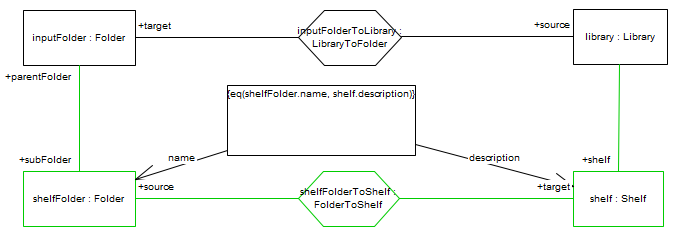
\includegraphics[width=\textwidth]{ea_completeForAllShelves}
  \caption{completed ForAllShelves}
  \label{ea:ForAllShelves_Complete}
\end{center}
\end{figure}

\item[$\blacktriangleright$] Now, we could have included a third, fourth, or tenth node element connected to \texttt{dictionary}, but that would force the
dictionary to have that many elements \emph{every} time. Even if it permitted up to ten, and your tree model only had 9, it would still fail for missing that
final partition.

\begin{figure}[htbp]
\begin{center}
  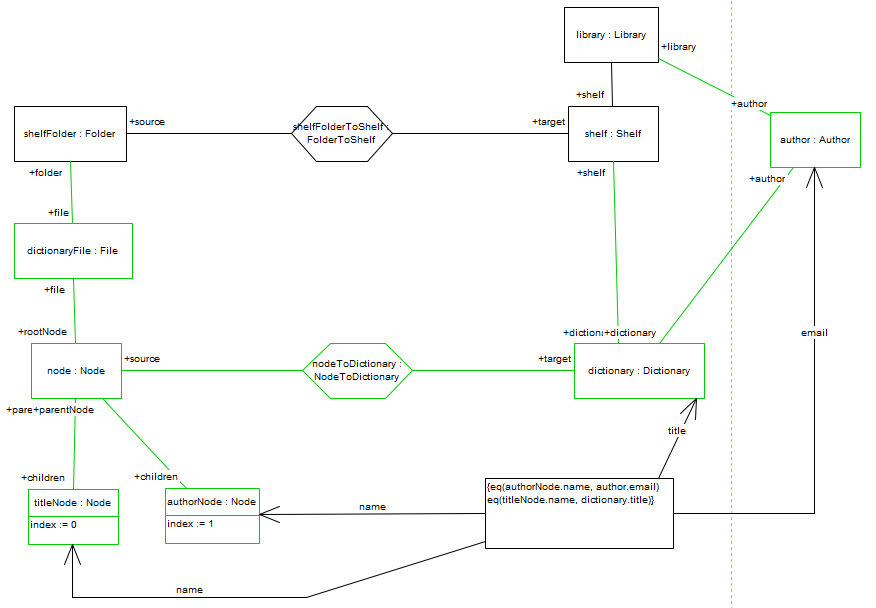
\includegraphics[width=\textwidth]{ea_completeNodeToDictionary}
  \caption{completed NodeToDictionary}
  \label{ea:NodeToDictionary_Complete}
\end{center}
\end{figure}

\item[$\blacktriangleright$] Let's handle the elements below. Similar logic as to \texttt{ForAllShelves} : links and specific context. This is how THAT also
handles multiples.

\begin{figure}[htbp]
\begin{center}
  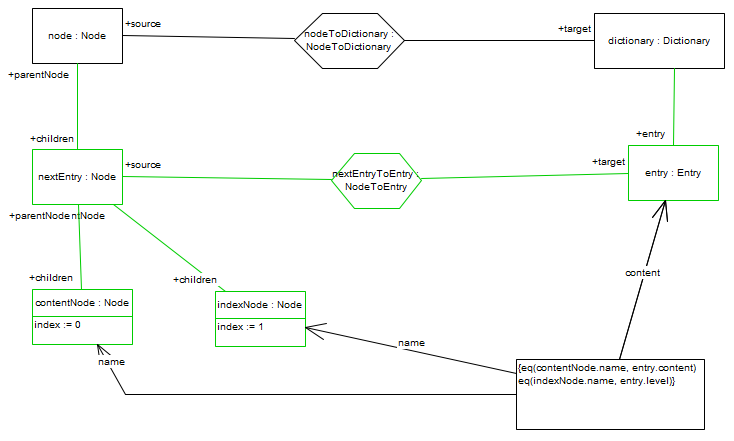
\includegraphics[width=\textwidth]{ea_completeForAllEntry}
  \caption{completed ForAllEntry}
  \label{ea:ForAllEntry_Complete}
\end{center}
\end{figure}

\item[$\blacktriangleright$] Validate: if you're having trouble exporting, try updating your schema first with any missing elements you may have created on the
fly. it should resemble\ldots

\begin{figure}[htbp]
\begin{center}
  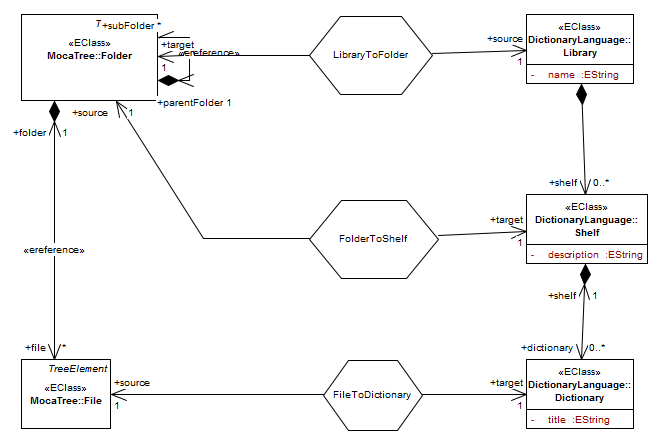
\includegraphics[width=\textwidth]{ea_completeSchema}
  \caption{completed Schema}
  \label{ea:Schema_Complete}
\end{center}
\end{figure}



\end{itemize}


